\documentclass[tikz,border=3.14mm]{standalone}
\begin{document}
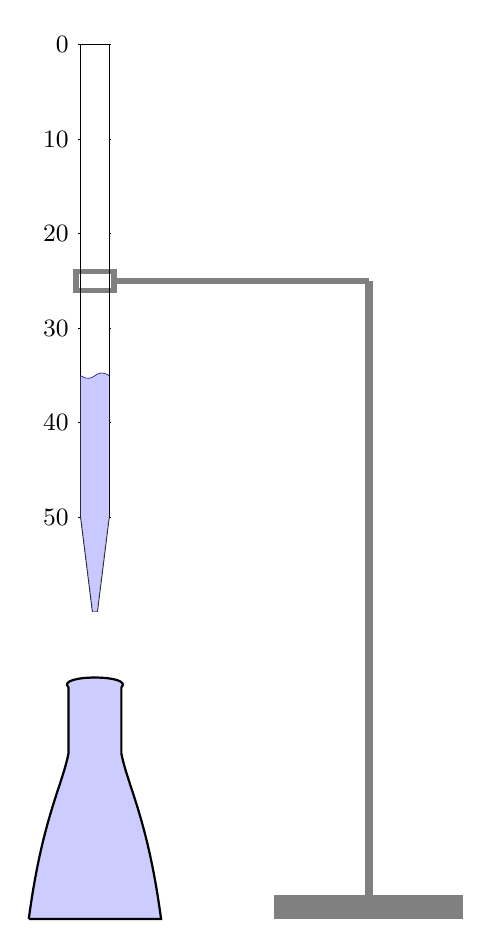
\begin{tikzpicture}[scale=0.6]

% Iron stand base (shifted right to accommodate longer horizontal arm)
\fill[black!50] (4.3,-8) rectangle (8.3,-8.5); % Base moved to x=5.3 (previously at x=2)

% Vertical rod (shifted right)
\draw[line width=3pt, black!50] (6.3,-8) -- (6.3,5); % Rod at x=6.3 (center of the new base)

% Extended horizontal arm
\draw[black!50, line width=2pt] (6.3,5) -- (0.9,5); % Arm spans from x=6.3 to x=0.9 (4.4 units)

% Clamp (unchanged position to stay attached to burette)
\draw[black!50, line width=2pt] (0.1,4.8) rectangle (0.9,5.2);

% Burette components (unchanged)
\draw (0.2,0) -- (0.2,10);
\draw (0.8,0) -- (0.8,10);
\draw (0.2,10) -- (0.8,10);

% Bottom taper
\draw (0.2,0) -- (0.45,-2);
\draw (0.8,0) -- (0.55,-2);
\draw (0.45,-2) -- (0.55,-2);

% Graduations (major)
\foreach \y/\label in {10/0,8/10,6/20,4/30,2/40,0/50}
{
  \draw (0.2,\y) -- (0.15,\y) node[left] {\small\label};
  \draw (0.8,\y) -- (0.85,\y);
}

% Graduations (minor)
\foreach \y in {1,3,5,7,9}
{
  \draw (0.2,\y) -- (0.175,\y);
  \draw (0.8,\y) -- (0.825,\y);
}

% Liquid (unchanged)
\fill[blue!30,opacity=0.7] (0.45,-2) -- (0.2,0) -- (0.2,3) .. controls (0.5,2.8) and (0.5,3.2) .. (0.8,3) -- (0.8,0) -- (0.55,-2) -- cycle;

% Meniscus highlight
\draw[blue!50!black,very thin] (0.2,3) .. controls (0.5,2.8) and (0.5,3.2) .. (0.8,3);

% Conical flask under the burette (scaled to twice the original size)
\begin{scope}[shift={(0.5,-8.5)}, scale=1.4]  % Scale changed from 0.7 to 1.4
    \draw[fill=blue!20, thick] (-1,0) -- (1,0) .. controls (0.8,1.5) and (0.5,2) .. (0.4,2.5) -- 
    (0.4,3.5) .. controls (0.6,3.7) and (-0.6,3.7) .. (-0.4,3.5) -- 
    (-0.4,2.5) .. controls (-0.5,2) and (-0.8,1.5) .. (-1,0);
\end{scope}

\end{tikzpicture}
\end{document}